\chapter{Web Application}
\todo[inline]{LP: zkuste to po sobe jeste precist. Pozor treba na jednotne/mnozne cislo (application vs. applications). Mit vetu pres 4 radky taky neni zrovna nejlepsi. Klidne se to da vic rozepsat. In this section, we will describe the proposed web application for novel song recommendation. The section is structured as follows:...

Celkove bude potreba, abyste se na to jeste podivala a zapracovala na preciznosti formulaci - muj pocit z te kapitoly je cca "no jako rozumim tomu, ale proc to proboha napsala takhle divne". Par prikladu jsem vyznacil nize v textu, ale je jich vic. Spis by stalo za to to poradne projit a prepsat - a ja na to mrknu detailneji az tohle probehne...}
In this section I will describe the features of the applications and the user interface in the \textbf{Analysis} section, the design chosen for this application with some high-level developer documentation in the \textbf{Design} section, possible developer configurations in the \textbf{Configuration possibilities} section and some high-level user documentation in the \textbf{User Documentation} section.

\section{Analysis}
\todo[inline]{LP: Takhle bohužel ne. Vy tady popisujete seznam naimplementovanych vlastnosti, tak by ale analyza fungovat nemela. Vy tu primarne chcete popsat, co uzivatel od vasi aplikace muze ocekavat - tasks a jakym zpusobem je chcete uchopit. Takze to co tu pisete je spise zaver analyzy, ale chybi k tomu nejaky uvod... Muzete take provest srovnani s jinymi systemy typu youtube/spotify a zakladni pozadavky uzivatelu od toho odvodit, pak pridat to cim se vymyka vas system - jde primarne o nalezeni noveho a jen o hudbu a na zaklade toho sestavit navrh implementovanych funkcionalit, pripadne i definovat dalsi pozadavky na system...}
The is in English \todo{LP: wtf?}. It requires users to create a unique username and password (there will also be a possibility of e-mail authentication - see section 6.3). For a logged in user, there are multiple functionalities. \\
From any page there are multiple redirection possibilities through a navigation bar. 
\begin{itemize}
    \item The \textit{Homepage} displays a truncated list of songs recommended to the current user. The user will also see a list of \textit{playlists} he created.
    \item The \textit{Recommended} page displays just a longer list of songs recommended to the user and also songs he played.
    \item The \textit{My lists} page displays all of the current users playlists along with first 10 songs and a list of songs recommended based on those in the particular list. From here, the user can create a new list or go to any \textit{List detail} page.
    \item The \textit{Add song} page is a form to add a new song. The lyrics and YouTube link are mandatory as well as the song and artist name. Songs added by any authenticated user are visible and recommendable to all the users. It is not possible to add a song that is already in the database.
    \item The \textit{All songs} page displays all songs that are in the database in ???alphabetical??? order.
    \item The \textit{Distance type} drop-down does not redirect the user to a different page but only changes the criteria for calculating and displaying recommended songs. The choices are based on the findings of this work: \begin{itemize}
        \item TF-idf
        \item Word2Vec
        \item \textit{??? Textova metoda ???}
        \item \textit{??? PCA}
        \item \textit{??? Neural network embedding}
    \end{itemize}
    \item The \textit{Search} input area and button search artists, songs titles and combination of those two based on what the user fills into the input area. The 10 best matches are displayed.
    \item The \textit{Username} drop-down lets the user log out.
\end{itemize}
There are also other redirection possibilities the user can access from only specific pages, not the navigation bar common for all the pages.
\begin{itemize}
    \item The \textit{Song detail} page displays an audio file where it is possible to play the song, songs most similar to this song (based on the users current distance-type selection), a possibility to \textit{like} or \textit{dislike} the song and also a \textit{add to a list} option.
    \item The \textit{List detail} page displays has the same structure as the \textit{Homepage}\todo{LP:. However,...} but instead of recommendations based on all songs, the recommendation is based only on songs from the particular list and also songs from the particular list are displayed.
    \item There are also possibilities to \textit{Add} and \textit{Delete} lists the user has created. No option like this for played songs though\todo[inline]{LP:Nonetheless, there are no options... (sentence fragment)}. Disliked songs do not appear in the played list listing. 
\end{itemize}
A simplified visualization of the request handling flow of the application is shown in Figure 6.1.

\begin{figure}[h]
    \centering
	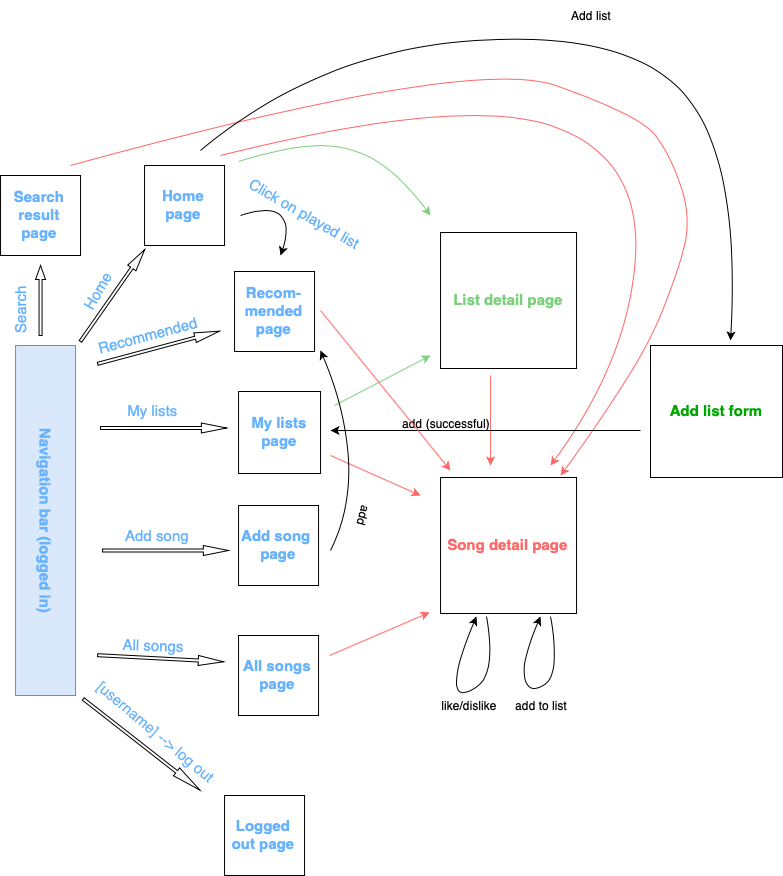
\includegraphics[height=120mm]{./img/analysis_diagram.png}
	\caption{Request diagram}
	\label{fig:analysis}
\end{figure}

\section{Design}
\todo[inline]{LP:Jak se na to divam, tak bych zmenil nazvy - tohle je spis Implementace a predchozi sekce - potom co ji dodelate by mohla byt analyza a design}
 To create the web application I used a web framework Django based on Python 3.7. The database used is PostgreSQL and to detach long computations that occur from user requests, I used the Celery asynchronous task queue with RabbitMQ as a broker.\\
 \todo[inline]{LP: Sem by se hodilo lehce popsat co jsou ty zminene technologie a proc jste si vybrala zrovna ty a ne neco jineho - jake jsou treba vyhody pythonu proti jinym variantam, proc zrovna celer s kralikem, co prinasi Django}
 The application consists of two main parts. The application itself (the client, server, models and views) and the similarity computation algorithms.
 
 \subsection{Application}
 
 \subsubsection{Client}
 
 The client has access to multiple html pages, all except of sign-up upon login. All the pages are Django templates written using HTML5 and some CSS for nicer design. \\
 
 The html pages \texttt{add\_song\_failed.html} \texttt{add\_to\_list\_failed.html}, \texttt{addSong.html}, \texttt{all\_songs.html} \texttt{index.html}, \texttt{list\_confirm\_delete.html} \texttt{list\_detail.html}, \texttt{list\_form.html}, \texttt{my\_lists.html}, \texttt{recommended\_songs.html}, \texttt{search\_results.html}, \texttt{song\_detail.html} these handle most of the interaction with the user and in-application functionalities. \\
 There are also special pages handling the user login and account \texttt{logged\_out.html, login.html, password\_reset\_complete.html, password\_reset\_confirm.html, password\_reset\_done.html, password\_reset\_email.html, password\_reset\_form.html, account\_activation\_email.html, account\_activation\_sent.html, signup.html}. \\
The page \texttt{base\_generic.html} is a base for all the html pages to keep the design consistent.

\subsubsection{Server}

The server does all the calculations in this application. To ensure a smooth user experience, the calculations are being sent to a task queue handled by Celery. This is possible because the computationally expensive requests users make do not need to be executed in a prescribed order. Those include:
\begin{itemize}
    \item adding a song, where the songs distance to all the songs in the database has to be computed for all the implemented distance-types of the application.
    \item liking and disliking songs as then the distance for all songs to the user and possibly to all lists the user has created needs to be recalculated
    \item adding a song to a list as all the other song distances to this list need to be recalculated
\end{itemize} 

\subsubsection{Database}

 The database is structured as the the Figure 6.2 displays.\todo[inline]{LP:The data structure is depicted on the Figure \ref{label obrazku} - takhle byste se z toho zblaznila, psat to vsechno rucne:-)} The user-related tables Django \todo{LP:tahle veta je trochu divna} automatically generates are omitted. The key tables are the \textit{Song}, \textit{Distance}, \textit{Profile} and \textit{List} table that store the main object the application uses. The others are there mostly to make make the system more clear and give easier access to desired objects. More specific description is provided in the \textbf{Model} section (6.2.?)
\begin{figure}[ht]
    \centering
	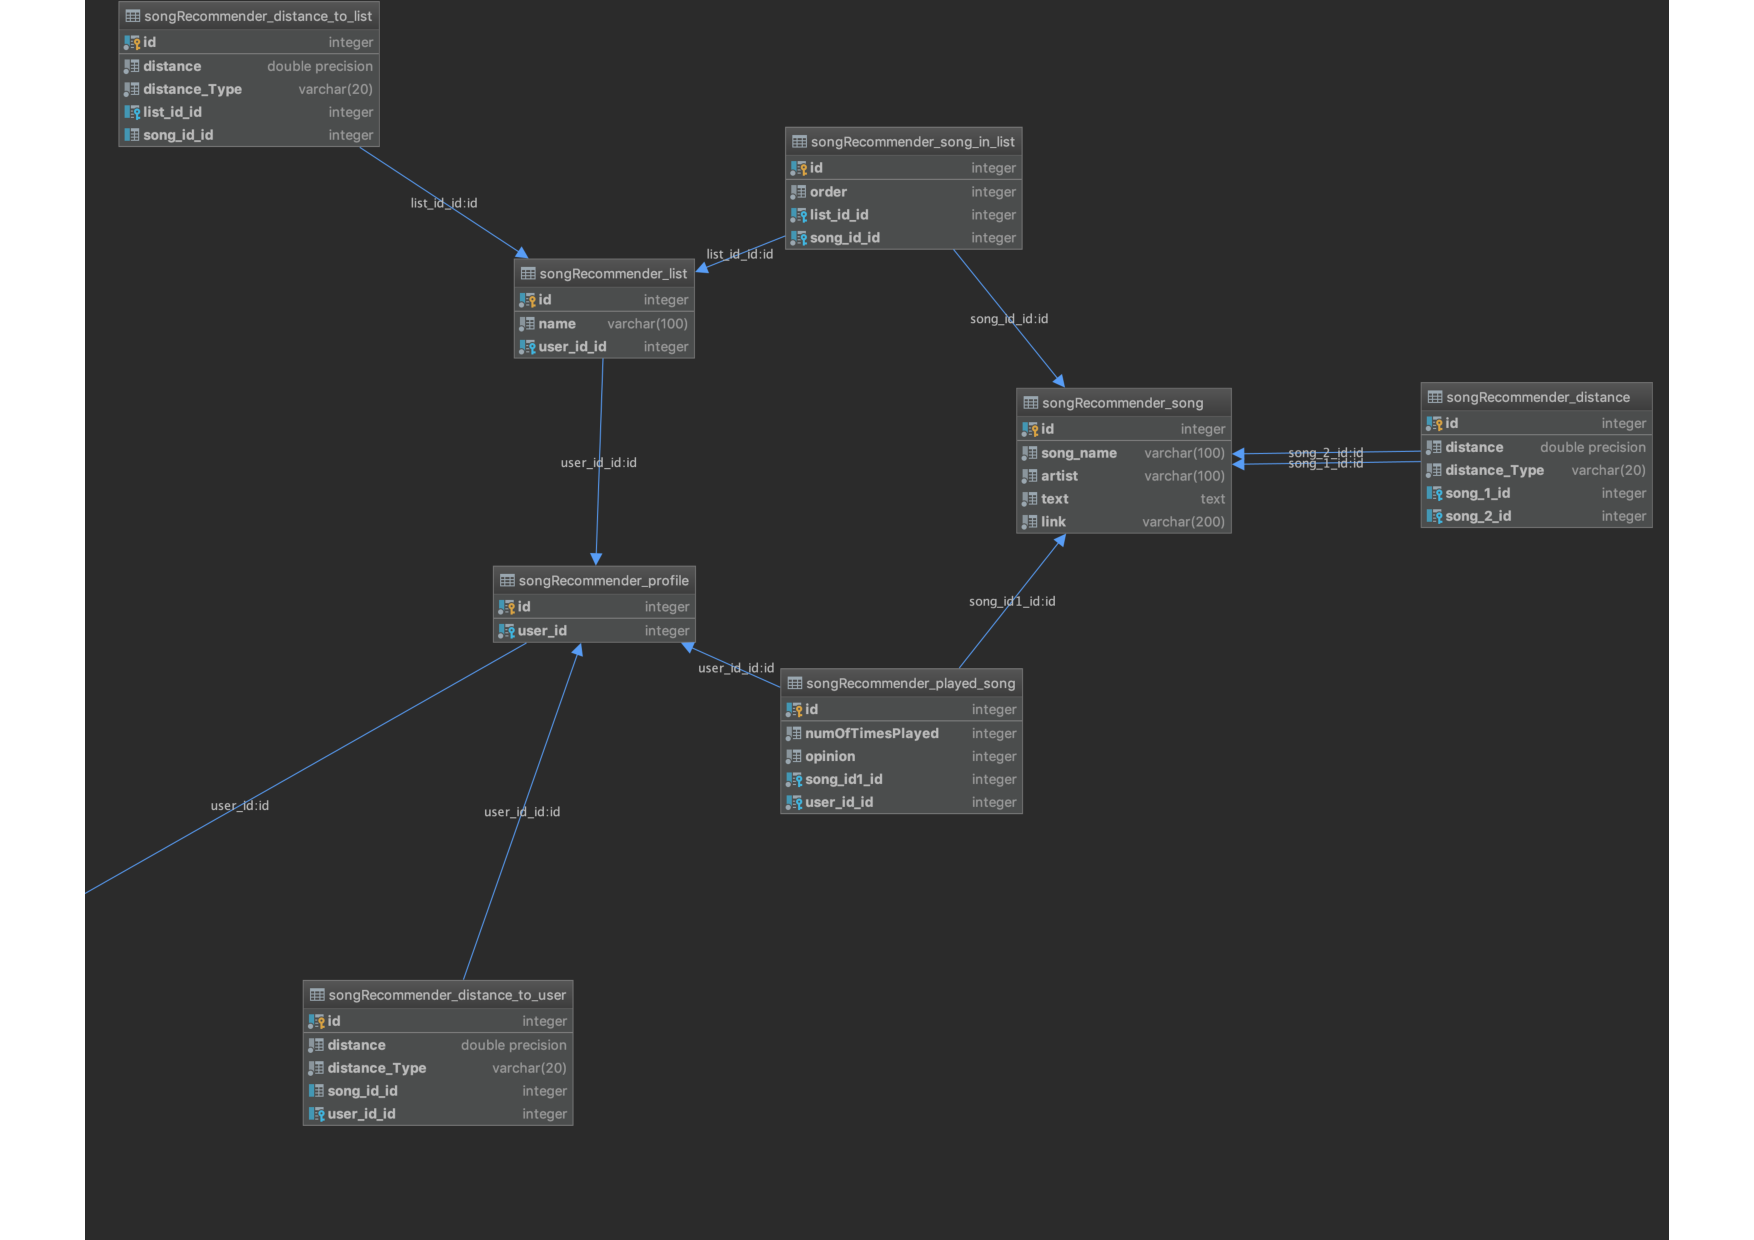
\includegraphics[width=120mm]{./img/database_diagram.pdf}
	\caption{Diagram of the applications database}
	\label{fig:diagram}
\end{figure}
 
 \subsubsection{Models}
 
 For every table in the database, there is a class-based model in the module \texttt{models.py} specifying their features. There is a class of the same name for \texttt{Song} and \texttt{List} table. The \texttt{Profile} model which is an extension of the build-in \texttt{User} model is included to enable specifying the distance of songs to the user and also checking if the user has confirmed his email.\\
 
The class \texttt{Song\_in\_list} keeps track of lists and songs that belong together, the model \texttt{Played\_song} specifies a user and all the songs he has played. One cannot un-play a song but it can be disliked and it will not appear anymore. \\

There are three different distance classes corresponding not to the way there were computed but corresponding to what distance they measure.\todo{LP: zase jedna divna veta.} First, the basic \texttt{Distance} class is the only class that actually stores distance based on a calculation of a similarity measurement algorithm. The classes \texttt{Distance\_to\_user} and \texttt{Distance\_to\_list} then calculate their distance data based on what they find in the \texttt{Distance} table using an algorithm from the module \texttt{tasks.py}.
 
\subsubsection{Views}

Views manage most of the data collection and send them as context to the html pages. There is one view for basically every html page plus some additional ones for some build in features for example liking and disliking songs, adding songs to lists etc. \\

The \texttt{HomePageView}, \texttt{MyListsView}, \texttt{AllSongsView} and \texttt{RecommendedSongsView} are build in Django list views with special features displaying query-sets from the database. As the names suggest they display the \textit{Homepage}, \textit{All songs} page, \textit{Recommended} page and \textit{My lists} page described in section 6.1. \\

The \texttt{ListDetailView} and \texttt{SongDetailView} are also Django build in views, for displaying detail pages of models from the database. They take care of displaying the detail page of a song and a list. \\

For the list, the creation, updating and deletion is also begin handled by build in views \texttt{ListUpdate}, \texttt{ListCreate} and \texttt{ListDelete}. \\

The rest is function based. Each corresponds each to some feature of the web application. 
\begin{itemize}
\item The \texttt{like} and \texttt{dislike} views manage liking and disliking songs.
\item The \texttt{add\_song} view handles adding songs to the database. This can be done by any logged in user and it results into the calculation all distances between the added song and all in the database.
\item The view \texttt{add\_song\_failed} handles if the user is trying to add a song that is probably already in the database.
\item The view \texttt{change\_distance} is called when the user decides to change the similarity measurement algorithm based on which songs are recommended to him.
\item The \texttt{search} view handles searching and displaying user song searches. 
\item The \texttt{signup},  \texttt{activate}, \texttt{account\_activation\_sent} and \texttt{logout} view handle user creation and authentication if email authentication is enabled.
\item The last two are \texttt{add\_song\_to\_list} and \texttt{add\_to\_list\_failed} which handle adding songs to lists.
\end{itemize}
 
 \subsection{Recommendation algorithms}
 \todo[inline]{LP: pozor na terminologii: Recommender systems / Recommending algorithms / Recommendation}

\section{Configuration possibilities}
\todo[inline]{LP: config. options}
\section{User documentation}